\section{Performance Analysis}\label{sec:performance analysis}
To test the performance of my code I designed two scripts which automated my
analysis. In the file \textit{test\_population.sh} there is code for running 10
runs of my code with population sizes from 10 to 100. The code uses different
random variables so we can get a proper average. The other settings was
"cross\_rate=1.0", "cover\_rate=0.5", "mutation=0.025", "elite=3" which means that it has a one point
crossover, approximately one mutation per gene and the 3 best\footnote{If this is
possible, for some population sizes this means that only the best are used
further} are used for the next population no matter what. I then use another script
\textit{average.py} to take the average over all which is then plotted using
\textit{plot\_population\_average.gnuplot}. In figure
\ref{fig:population-average} you can see the result of all the runs\footnote{In
	many of the plots there is no standard deviation or average plotted,
	this is done because including them would mean so much clutter that it
would be impossible to interpret anything useful from the plots}.

\begin{figure}[h!]
	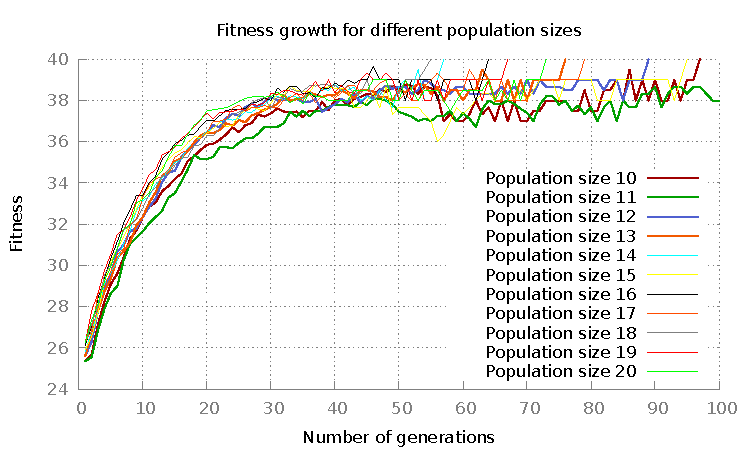
\includegraphics{../graphs/fitness_population_average.pdf}
	\caption{Average fitness growth for the best individual for different populations}
	\label{fig:population-average}
\end{figure}

As can be seen from the plot there is no clear winner, several reaches the max
fitness within 100 generations and some don't. This is also dependant on the
random seed selected. For this reason I will continue forward with a population
size of 40, because I'm quite sure that it should always make it. Although this
is very hard to say as it seem that with the current configuration it is all
rather random if it makes it or not, but as one can see 40 makes it. This means
that 40 has done well over 10 runs with a new random seed each time.

When testing for crossover and mutation rate the task was a bit more difficult
to plot concise. For this reason I made a another script,
\textit{test\_crossover.sh}, which can test a lot of different mutation and
crossover rates. The problem is plotting this. I haven't found a pretty way of
showing it, so below I include two out of seven plots\footnote{There should be
no problem recreating the results and looking at them}, one containing the best
results and one other which show another good configuration. For the plots I have run
10 times with different seeds for each of the 10 times, but the same seed for
different crossovers and mutation rates. I used a population size of 40 as said
above and elitism of 3 to keep it consistent with the test ran above.

\begin{figure}[h!]
	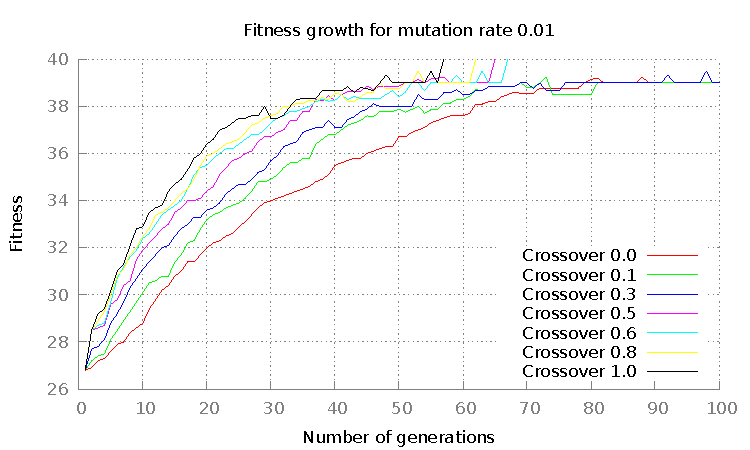
\includegraphics{../graphs/fitness_crossover_mute_001_average.pdf}
	\caption{Average fitness for the best individual with a mutation rate of 0.01 and all the
	different crossover rates tested for}
	\label{fig:cross 0.01}
\end{figure}

\begin{figure}[h!]
	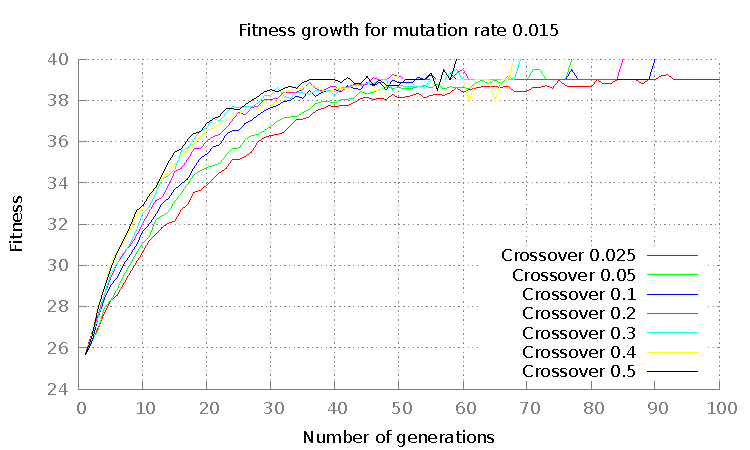
\includegraphics{../graphs/fitness_crossover_mute_0015_average.pdf}
	\caption{Average fitness of the best individual with a mutation rate of
		0.015 and all the different crossover rates tested for}
	\label{fig:cross 0.015}
\end{figure}

In figure \ref{fig:cross 0.01} we can see that with a crossover rate of 1.0 and
a mutation rate of 0.01 we can solve the \textit{One-Max problem} in around 57
generations\footnote{This was the lowest of all the seven runs, but random seed
	will affect this, so this might not be exactly the same for other
runs, but I think that average of 10 runs should yield good results}. To
extrapolate from this is quite hard, but it seems that a large crossover rate
and a low mutation rate is better than the other way around. This seem to
suggest that inheritance is very important, and a low chance of mutation with
few major changes to the gene is good. This would correlate well with what we
have learned in class about evolutionary algorithms.

\subsection{Selection Mechanism}\label{sec:selection mechanism}
When testing for the best selection mechanism I again started by making a new
script for automated testing, \textit{test\_selection.sh}. This files run
through all of the different selection mechanisms that I have implemented,
namely \textit{Fitness Proportionate}, \textit{Sigma Scaling}, \textit{Rank
Selection} and \textit{Tournament Selection}. The result can be seen below in
figure \ref{fig:selection}. In ran with the parameters found in the previous
section and with tournament size on 10 and the e factor on 0.05 which where both
chosen after some testing\footnote{This was not the most extensive testing so
Tournament selection might improve more}.

\begin{figure}[h!]
	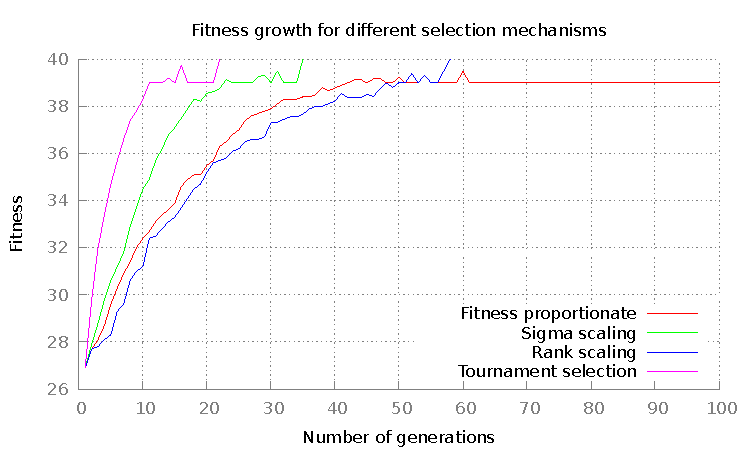
\includegraphics{../graphs/fitness_selection_average.pdf}
	\caption{Average fitness of the best individuals with different
	selection mechanisms}
	\label{fig:selection}
\end{figure}

In the figure we can see that Tournament selection does a remarkably good job
compared to Fitness Proportionate, Sigma scaling also does a good job and rank
selection does improve compared to Fitness Proportionate.

\subsection{Random Target}\label{sec:random target}
For this task I ran a new script which generated 40bit long random strings and
ran four different tests, again with 10 different runs. In figure
\ref{fig:random target} we can see the results. If we compare this with the
results obtained in figure \ref{fig:target one max} we can see that there really is
not that much difference between them\footnote{Both of these runs had the exact
	same premises which should mean that very little is different between
	them. One problem is that this is the average over four different random
	bit strings. Another problem is the inherent randomness which comes with
the testing. I ran a couple of times and was quite ready to call One-Max easier,
but than I got a couple of results like the ones below and it again switched for
me.}. Even tough it is a bit quicker in figure
\ref{fig:random target} that can easily be attributed to random and as such I
conclude that trying to evolve a random target is no different from an all one
target. This makes sense since in many ways an all one target is no different
from a randomly chosen different bit string. As an example say we have a random
target which must have a "101" somewhere inside and a random phenotype in the
population which contains "111" converting between those two are no different from the
one max problem going the other way, and as such is no different.

\begin{figure}[h!]
	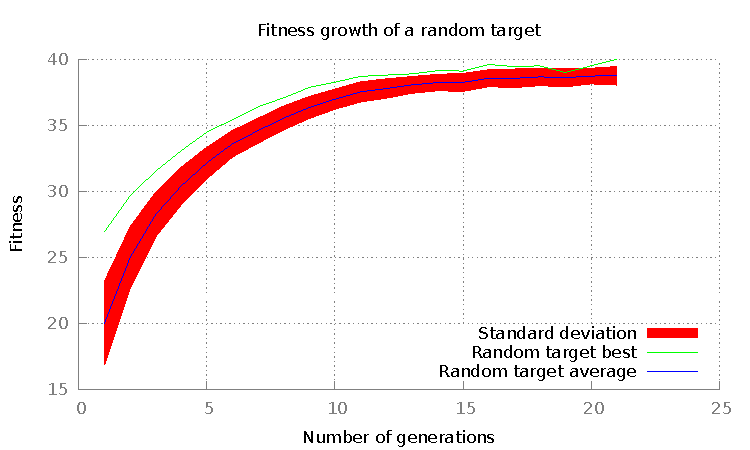
\includegraphics{../graphs/fitness_target_random.pdf}
	\caption{Averaged values of four different randomly selected targets and
	with average, best and standard deviation.}
	\label{fig:random target}
\end{figure}

\begin{figure}[h!]
	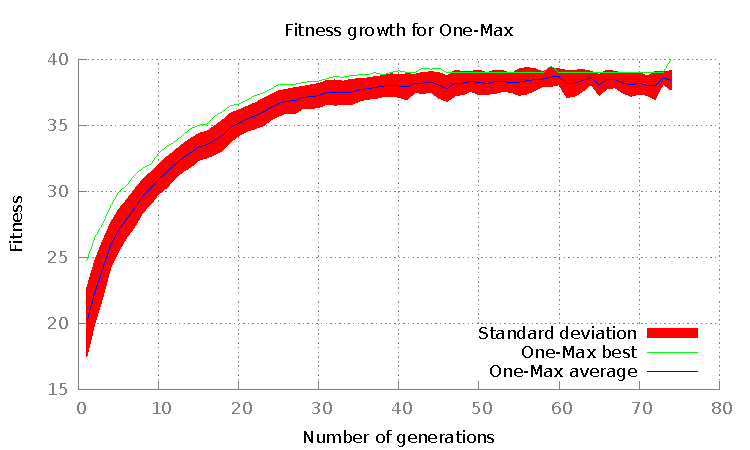
\includegraphics{../graphs/fitness_target_one.pdf}
	\caption{Averaged values for the One-Max problem 
	with average, best and standard deviation.}
	\label{fig:target one max}
\end{figure}
